\documentclass{article}
\usepackage{arxiv}
\usepackage[utf8]{inputenc}
\usepackage[english, russian]{babel}
\usepackage[T1]{fontenc}
\usepackage{url}
\usepackage{booktabs}
\usepackage{amsfonts}
\usepackage{nicefrac}
\usepackage{microtype}
\usepackage{lipsum}
\usepackage{graphicx}
\usepackage{natbib}
\usepackage{doi}


\title{Классификация товаров по ОКПД2 кодам}

\author{ Фирсов Сергей \\
        Кафедра интеллектуальных систем\\
	МФТИ\\
	\texttt{firsov.sa@phystech.edu} \\
	\And
	Всеволод Михайлович Старожилец \\
	Кафедра интеллектуальных систем\\
	Форексис\\
	\texttt{vsevolod.starozhilets@antirutina.net} \\
	%% \AND
	%% Coauthor \\
	%% Affiliation \\
	%% Address \\
	%% \texttt{email} \\
	%% \And
	%% Coauthor \\
	%% Affiliation \\
	%% Address \\
	%% \texttt{email} \\
	%% \And
	%% Coauthor \\
	%% Affiliation \\
	%% Address \\
	%% \texttt{email} \\
}
\date{}

\renewcommand{\shorttitle}{\textit{arXiv} Template}

%%% Add PDF metadata to help others organize their library
%%% Once the PDF is generated, you can check the metadata with
%%% $ pdfinfo template.pdf
\hypersetup{
pdftitle={Декодирования сигналов головного мозга в аудиоданные},
pdfsubject={q-bio.NC, q-bio.QM},
pdfauthor={Набиев Мухаммадшариф, Северилов Павел},
pdfkeywords={First keyword, Second keyword, More},
}

\begin{document}
\maketitle

\begin{abstract}
    Исследование направлено на решение задачи классификации товаров по кодам Общероссийского классификатора продукции по видам экономической деятельности (ОКПД 2) с использованием кратких текстовых описаний. Коды представляют собой детализированную систему категоризации продуктов и услуг по видам экономической деятельности. Основная цель --- повышение точности и сокращение ресурсозатратности классификации, за счёт анализа влияния глубины ОКПД 2. Для достижения этих целей предлагается метод построения текстовых эмбеддингов с использованием нейросетевых технологий. Задача усложняется необходимостью предварительной обработки данных для перевода исходных описаний в стандартизированные короткие тексты, адаптированные для анализа. Используются данные государственных закупок по ФЗ 44 за 2022 год. Новизна работы заключается в применении методов машинного обучения к индустриальной задаче, что обещает улучшение в процессах логистики, учёте и анализе в сфере закупок. 


 
\end{abstract}


\keywords{OKPD 2 code \and text analysis \and task of classification}

\section{Введение}

Целью данного исследования является разработка и апробация метода классификации товаров по кодам ОКПД 2 (\cite{OKPD2024}), используя краткие текстовые описания. Актуальность задачи обусловлена необходимостью повышения эффективности процессов логистики и учета в сфере закупок, а также сокращения времени и ресурсов, затрачиваемых на классификацию товаров.

Объектом исследования выступают любые товары, для которых возможна классификация по ОКПД 2 кодам (детализированной системе категоризации продукции и услуг по видам экономической деятельности). Проблема заключается в разработке метода, позволяющего автоматизировать этот процесс с высокой точностью и полнотой классификации, устойчиво относительно формата входных данных, и в исследовании характеристик этого метода (по указанным параметрам) от глубины классификации.

Задача классификации по кодам разобрана здесь (добавить). В дальнейшей работе также будем опираться на курс лекций Воронцова К.В. и книги \cite{Goodfellow2016DeepLearning} и \cite{Montani2019AdvancedNLP}. %
%нужно найти и вставить нормальные статьи про классификацию кодов (9)  
Текстовый эмбеддинг --- веторное представление слова. Вектора отражают семантическое значение каждого слова на основе контекста. Наиболее часто они получаются при помощи методов Word2Vec  или GloVe.  Эти методы используют нейронные сети и стараются либо предугадать пропущеное слово по контексту, либо восстановить контекст по слову. Опираемся на эти статьи: \cite{alammarWord2vec} и \cite{munozWordEmbeddings}.  
Мы пользуемся библиотекой spaCy \cite{spacyDocs}, основанной на вышеописанных методах и имеющей предобученные модели, готовые для взаимодействия с русским языком и короткими текстами. После построения эмбендингов --- решаем задачу классификации, сопоставляем вектора и классы ОКПД 2.  Дальше исследуем качество классификации варьируя глубину классификатора --- что и есть основная суть исследования. 

Используются данные государственных закупок по ФЗ 44 за 2022 год. Это позволяет оценить работу алгоритма в условиях большого объема и разнообразия данных. Исследование включает в себя подготовку данных, построение модели классификации и ее тестирование с целью определения оптимальных параметров для достижения максимальной точности классификации в зависимости от необходимой глубины класификации. Рабочий процесс описывает последовательные шаги от предварительной обработки текстов до оценки результатов классификации.

В заключение, данное исследование представляет собой вклад в развитие методов машинного обучения и их применение к решению практических задач классификации товаров, что имеет важное значение для сферы государственных закупок и управления цепочками поставок.

\section{Постановка проблемы}
Дана выборка для задачи многоклассовой классификации, с количеством классов $K$:

$$\mathfrak{D}  = \{(\bold{x}_i, y_i)\}_{i=1}^{m},\; \bold{x}_i = \text{text \ description},\; y_i \in \mathbb{Y}  = \{1, \dots, K\},$$

Выборка разбита на обучающую и тестовую части: $\mathfrak{D} = \mathfrak{D}_\text{train} \bigsqcup \mathfrak{D}_\text{test}$.

Будет использоваться линейная модель классификации, $A = \{ \ g(x,\theta) \ | \ \theta \in \mathcal{R} \ \}$ , где $g(x, \theta) = sign \sum \limits_{j=1}^n \theta_j f_j(x)$.

Используется квадратичная функция потерь: $\mathcal{L}(a,x) = (a(x) - y(x))^2$, где $y$ --- значения контрольной выборки.  

Откуда получаем функцию Эмпирического риска : $Q(a,X^l)=\frac{1}{l}\sum\limits^l_{i=1}\mathcal{L}(a,x_i)$

И будем решать задачу оптимизации --- минимизации эмпирического риска 
$$ \mu(X^l) = arg \min_{a\in A} Q(a, X^l)$$


Критерий качества в задаче нашей классификации - попадание конкретного товар в свою категорию и в правильный ОКПД 2 код.


\section{Планирование вычислительного эксперимента}

Цель эксперимента --- исследование алгоритма классификации, построенного с помощью текстовых эмбендингов, в зависимости от глубины классификации.

Выборка данных из госзакупок, представляет собой набор объектов --- текстовых описаний товаров, и их признаков --- код их ОКПД2 классификации. Описания некоторых товаров слишком специфичны, для чего их укоротили и стандартизировали. %to be done  

Пример итогового описания и кода: Яйца куриные в скорлупе свежие	01.47.21.000  

Выборка разделена на обучающую и тестовую часть, размерами 6 и 2 миллиона записей соответственно.  

Используя sklearn и spaCy строятся сначала текстовые эмбендинги для слов, далее по ним решается задача классификации. Варьируется необходимая глубина классификации и исследуется в зависимости от этого количество ошибок при классификации.

Таблицы - точность алгоритма в зависимости от ступени класификатора: 
в процентном соотношении для 1,2,3,4 ступени.
Груфик по этой таблице.

\section{Базовый алгоритм}
Для базового алгоритма выбрана лог регресия.  
В качестве набора данных взята часть выборки --- первый миллион записей. По ним строятся эмбендинги и с помощью sklearn решается задача лог регрессии. По полученным результатам строим ROC кривую.

Код и сама выборка находятся в соответствующих файлах проекта.

Здесь ROC кривая для первого класса после классификации:
\begin{figure}[h]
\centering
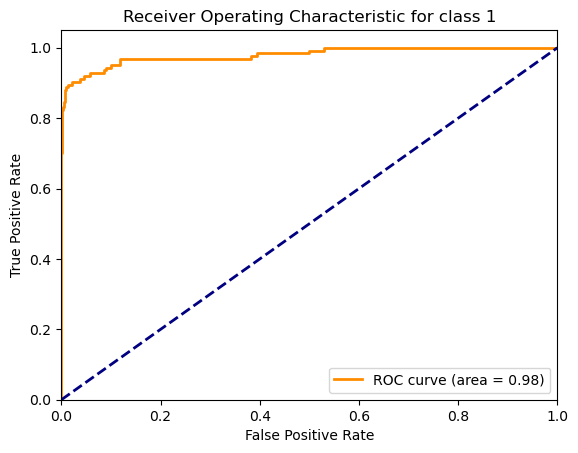
\includegraphics[width=0.8\linewidth]{roc_1.png}
\caption{ROC кривая для одного из классов после базового эксперимента}
\label{fig:mpr}
\end{figure}

\bibliographystyle{unsrtnat}
\bibliography{Firsov2024Classification_according_to_OKPD_2_codes}

\end{document}